\begin{pastexam}[label={px:ust-113-ee-ds-20}]{臺聯大電機類 113 學年度 問答題第 4 題}
（問答；10 分）

Given the following codes, please answer the three questions:
\begin{enumerate}[label=(\Alph*)]
\item What should be filled in Q1 and Q2 (4 points)
\item Which traverse order does the codes implement for? (3 points.)
\item What is the output of the codes? (3 points.)
\end{enumerate}
\begin{minted}[fontsize=\small, style=perldoc, breaklines]{java}
class Node {
    int key;
    Node left, right;
    public Node(int item) {
        key = item;
        left = right = null;
    }
}
public class BinarySearchTree {
    Node root;
    BinarySearchTree() {
        root = null;
    }
    void insert(int key) {
        root = insertRec(root, key);
    }
    Node insertRec(Node root, int key) {
        if (root == null) {
            root = new Node(key);
            return root;
        }
        if ( Q1 )
            root.left = insertRec(root.left, key);
        else if ( Q2 )
            root.right = insertRec(root.right, key);
        return root;
    }
    void order() {
        orderRec(root);
    }
    void orderRec(Node root) {
        if (root != null) {
            orderRec(root.left);
            System.out.print(root.key + " ");
            orderRec(root.right);
        }
    }
    public static void main(String[] args) {
        BinarySearchTree tree = new BinarySearchTree();
        tree.insert(5);
        tree.insert(3);
        tree.insert(2);
        tree.insert(4);
        tree.insert(7);
        tree.insert(6);
        tree.insert(8);
        tree.order();
    }
}
\end{minted}
\end{pastexam}

\begin{pastsoln}
\textbf{(A)} Q1：\texttt{key < root.key}；Q2：\texttt{key > root.key}。

二元搜尋樹的插入（資結書第~9.2~節、虛擬碼~9.6）：比目前節點小往左子樹插，比較大往右子樹插，走到空的
位置建新節點。 \texttt{insertRec} 回傳插入後這棵子樹的根，呼叫端用它更新 \texttt{root.left} 或
\texttt{root.right}，所以空子樹也接得上。 兩個條件都不成立就是 \texttt{key == root.key}，什麼都不做，
直接回傳：重複的鍵不插入。 （Q2 也可以寫 \texttt{key >= root.key} 讓重複的鍵放右邊，但既然有
\texttt{else if}，原本的意思是排除相等的情形。）

\textbf{(B)} 中序走訪（inorder）：\texttt{orderRec} 先走左子樹、再印自己、再走右子樹（資結書第~7.3~節）。

\textbf{(C)} 依序插入 $5, 3, 2, 4, 7, 6, 8$：$5$ 是根；$3 < 5$ 在左；$2$ 在 $3$ 左；$4$ 在 $3$ 右；$7 > 5$
在右；$6$ 在 $7$ 左；$8$ 在 $7$ 右。

\begin{center}
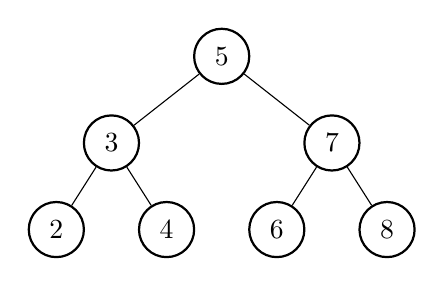
\begin{tikzpicture}[every node/.style={circle, draw, thick, minimum size=7mm, inner sep=0pt},
    level distance=11mm, level 1/.style={sibling distance=28mm}, level 2/.style={sibling distance=14mm}]
\node {5}
  child {node {3} child {node {2}} child {node {4}}}
  child {node {7} child {node {6}} child {node {8}}};
\end{tikzpicture}
\end{center}

BST 的中序就是由小到大（資結書定理~9.1），輸出
\begin{center}
\texttt{2 3 4 5 6 7 8 }
\end{center}
（每個數後面都有一個空格，最後也有。）
\end{pastsoln}
